%!TEX root = ../out/10-TW-SL.tex


\begin{document}
	
\title[Treewidth]
{Parameter Treewidth}

\begin{frame}
  \titlepage
\end{frame}

\lecturenotes{\maketitle}

\begin{frame}
 \slides{\frametitle{Outline}}
 \tableofcontents
\end{frame}

\section{Algorithms for trees}

\begin{frame}
 \frametitle{Exercise}
 
  \noindent
 	\textbf{Recall}: An \alert{independent set} of a graph $G=(V,E)$ is a set of vertices $S\subseteq V$ such that $G[S]$ has no edge.
 	
        \pbDefOpt{\#\textsc{Independent Sets on Trees}}{A tree $T=(V,E)$}{The number of independent sets of $T$.}
        
        \begin{itemize}
         \item Design a polynomial time algorithm for \#\textsc{Independent Sets on Trees}
        \end{itemize}

\end{frame}


\newcommand{\nbin}{\ensuremath{\mathsf{\#in}}}
\newcommand{\nbout}{\ensuremath{\mathsf{\#out}}}
\newcommand{\nboutD}{\ensuremath{\mathsf{\#outD}}}
\newcommand{\nboutND}{\ensuremath{\mathsf{\#outND}}}


\begin{frame}{Solution}
	\begin{itemize}
		\item Select an arbitrary root $r$ of $T$
		\item Bottom-up dynamic programming (starting at the leaves) to compute, for each subtree $T_x$ rooted at $x$ the values
		\begin{itemize}
			\item $\nbin(x)$: the number of independent sets of $T_x$ containing $x$, and
			\item $\nbout(x)$: the number of independent sets of $T_x$ not containing $x$.
		\end{itemize}
		\item If $x$ is a leaf, then $\nbin(x)=\nbout(x)=1$
		\item Otherwise,
		\begin{align*}
		 \nbin(x) &= \Pi_{y \in \text{children} (x)} \;\nbout(y) \text{ and}\\
		 \nbout(x) &= \Pi_{y \in \text{children} (x)} \;(\nbin(y)+\nbout(y))
		\end{align*}
		\item The final result is $\nbin(r)+\nbout(r)$
	\end{itemize}
\end{frame}


\begin{frame}
 \frametitle{Exercise}
 
  \noindent
 	\textbf{Recall}: A \alert{dominating set} of a graph $G=(V,E)$ is a set of vertices $S\subseteq V$ such that $N_G[S]=V$.
 	
        \pbDefOpt{\#\textsc{Dominating Sets on Trees}}{A tree $T=(V,E)$}{The number of dominating sets of $T$.}
        
        \begin{itemize}
         \item Design a polynomial time algorithm for \#\textsc{Dominating Sets on Trees}
        \end{itemize}

\end{frame}


\begin{frame}{Solution}
	\begin{itemize}
		\item Select an arbitrary root $r$ of $T$
		\item Bottom-up dynamic programming (starting at the leaves) to compute, for each subtree $T_x$ rooted at $x$ the values
		\begin{itemize}
			\item $\nbin(x)$: the number of dominating sets of $T_x$ containing $x$,
			\item $\nboutD(x)$: the number of dominating sets of $T_x$ not containing $x$, and
			\item $\nboutND(x)$: the number of vertex subsets of $T_x$ dominating $V(T_x)\setminus \{x\}$.
		\end{itemize}
		\item If $x$ is a leaf, then $\nbin(x)=\nboutND(x)=1$ and $\nboutD(x)=0$.
		\item Otherwise, 
		\begin{align*}
		 \nbin(x) &= \Pi_{y \in \text{children} (x)} \; (\nbin(y)+\nboutD(y)+\nboutND(y)),\\
		 \nboutD(x) &= \Pi_{y \in \text{children} (x)} \; (\nbin(y)+\nboutD(y))\\ &\quad - \Pi_{y \in \text{children} (x)} \; \nboutD(y)\\
		 \nboutND(x) &= \Pi_{y \in \text{children} (x)} \; \nboutD(y)
		\end{align*}
		\item The final result is $\nbin(r)+\nboutD(r)$
	\end{itemize}
\end{frame}

\section{Tree decompositions}

\begin{frame}
  \frametitle{Algorithms using graph decompositions}
  
  
  \pgfdeclarelayer{background}
  \pgfsetlayers{background,main}
  \begin{tikzpicture}
  	\tikzstyle{set} = [color=Green,opacity=.2,line cap=round, line join=round, line width=19pt]
  	
  	\begin{pgfonlayer}{background}
  	  \draw[set] (0,0)--(0,1);
  	  \draw[fill=black] (0,0) circle (0.8mm);
  	  \draw[fill=black] (-0.1,1) circle (0.8mm);
  	  \draw[fill=black] ( 0.1,1) circle (0.8mm);
  	  \draw[set] (-0.05,-0.05)--(-0.2,-0.9);
  	  \draw[fill=black] (-0.25,-0.8) circle (0.8mm);
  	  \draw[fill=black] (-0.15,-1) circle (0.8mm);
  	  \draw[set] (0.05,-0.05)--(0.7,-0.7);
  	  \draw[fill=black] (0.7,-0.7) circle (0.8mm);
  	  \draw[set] (-0.2,-0.9)--(-1.2,-0.9);
  	  \draw[set] (0.7,-0.7)--(1.2,0);
      \draw[set] (-0.05,0.95)--(-0.2,1.9);
      \draw[fill=black] (-0.2,1.9) circle (0.8mm);
      \draw[set] (0.05,0.95)--(0.65,1.65);
      \draw[fill=black] (0.65,1.65) circle (0.8mm);
      \draw[set] (-0.2,1.9)--(-0.4,2.75);
      \draw[set] (0.65,1.65)--(0.75,2.6);
  	\end{pgfonlayer}
  \end{tikzpicture}  
  ~~%
  \begin{minipage}[b]{6cm}
    \emph{Idea:} decompose the problem into subproblems and combine solutions
    to subproblems to a global solution.

    \bigskip

    \emph{Parameter:} overlap between subproblems.
  \end{minipage}

\end{frame}





\begin{frame}[label=treedecomp,shrink=2]
  \frametitle{Tree decompositions (by example)}


  \begin{itemize}
  \item<1-> A graph $G$

\tikzstyle{set} = [color=Green,opacity=.15,line cap=round, line join=round, line width=18pt]
\pgfdeclarelayer{background}
\pgfsetlayers{background,main}
\begin{tikzpicture}[yscale=.5]

 \draw[thick] 
    (0,3) node[vertex,label=left:$a$] (a) {}
    (1,4) node[vertex,label=above:$b$] (b) {}
    (2,3) node[vertex,label=above:$c$] (c) {}
    (3,3) node[vertex,label=above:$d$] (d) {}
    (2,1) node[vertex,label=left:$e$] (e) {};
 \draw<1-4>[thick] 
    (3,1) node[vertex,label=below:$f$] (f) {};
 \draw<5->[thick] 
    (3,1) node[vertex,label=below:$\textcolor{red}{f}$] (f) {};
 \draw[thick] 
    (4,2) node[vertex,label=above:$h$] (h) {}
    (4,0) node[vertex,label=right:$g$] (g) {}
    (5,2) node[vertex,label=above:$i$] (i) {}
    (6,3) node[vertex,label=right:$j$] (j) {}
    (6,1) node[vertex,label=right:$k$] (k) {}

(b)--(c) (a)--(c) (e)--(f) (c)--(d) (f)--(g) (f)--(h) (c)--(d)
(c)--(e) (d)--(h) (f)--(h)--(i)--(j) (i)--(k) ;
 \draw<1-3>[thick] (a)--(b);
 \draw<4->[very thick,color=green!50!black] (a)--(b);
 
 \begin{pgfonlayer}{background}
\draw<2->[set] (a)--(b)--(c)--(a);
\draw<2->[set,color=Blue] (e)--(c)--(d);
\draw<2->[set] (e)--(f)--(d);
\draw<2->[set,color=Red] (f)--(g);
\draw<2->[set,color=Black] (d)--(h)--(f);
\draw<2->[set] (h)--(i);
\draw<2->[set,color=Blue] (j)--(i);
\draw<2->[set,color=Red] (k)--(i);
 \end{pgfonlayer}

\end{tikzpicture}


\item<2-> A \emph{tree decomposition} of $G$

  \begin{tikzpicture}[xscale=1.8]
    \draw<1-3>[thick,ellipse]
     (-0.5,0) node[draw,color=Green] (abc) {$a,b,c$};
    \draw<4->[thick,ellipse]
     (-0.5,0) node[draw,color=Green] (abc) {$\textcolor{green!50!black}{a},\textcolor{green!50!black}{b},c$};
    \draw<1-4>[thick,ellipse]
     (1.75,0) node[draw,color=Green] (def) {$d,e,f$}
     (3,0) node[draw] (dfh) {$d,f,h$}
     (1.75,-1) node[draw,color=Red] (fg) {$f,g$};
    \draw<5->[thick,ellipse]
     (1.75,0) node[draw,color=Green] (def) {$d,e,\textcolor{red}{f}$}
     (3,0) node[draw] (dfh) {$d,\textcolor{red}{f},h$}
     (1.75,-1) node[draw,color=Red] (fg) {$\textcolor{red}{f},g$};
    \draw[thick,ellipse]
     (0.5,0) node[draw,color=Blue] (cde) {$c,d,e$}
     (4,0) node[draw,color=Green] (hi) {$h,i$}
     (5,1) node[draw,color=Blue] (ij) {$i,j$} 
     (5,-1) node[draw,color=Red] (ik) {$i,k$}
     (abc)--(cde)--(def)--(dfh)--(hi)--(ij) (hi)--(ik) (def)--(fg);
  \end{tikzpicture}
  


  \only<3->{Conditions:} 
  \only<4->{\textcolor{green!50!black}{covering}}
  \only<5->{and \textcolor{red}{connectedness.}}


%  \only<6->{
%  \item Useful Observation: 
%  Let $G$ be a graph and $X\subseteq V(G)$. Then $\tw(G)\leq
%  \tw(G-X)+\Card{X}$.}
  \end{itemize}
\end{frame}


\begin{frame}
  \frametitle{Tree decomposition (more formally)}
  \begin{itemize}
  \item Let $G$ be a graph, $T$ a tree, and $\gamma$ a labeling
    of the vertices of~$T$ by sets of vertices of~$G$. 
  \item We refer to the
    vertices of $T$ as ``nodes'', and we call the sets $\gamma(t)$ ``bags''.
  \item The pair $( T, \gamma )$ is a \emph{tree decomposition} of~$G$ if
    the following three conditions hold:
    \begin{enumerate}
    \item For every vertex $v$ of $G$  there exists a node $t$ of $T$ 
      such that $v \in \gamma(t)$.
    \item For every edge $vw$ of $G$ there exists a node $t$ of $T$ such
      that $v,w \in \gamma(t)$ (``covering'').
    \item For any three nodes $t_1, t_2, t_3$ of $T$, if $t_2$ lies on
      the unique path from $t_1$ to~$t_3$, then $\gamma(t_1) \cap
      \gamma(t_3) \subseteq \gamma(t_2)$ (``connectedness'').
    \end{enumerate} 
  \end{itemize}    
\end{frame}


\begin{frame}
  \frametitle{Treewidth}
  \begin{itemize}
  \item The \emph{width} of a tree decomposition $( T, \gamma )$ is defined as
    the maximum $|\gamma(t)|-1$ taken over all nodes~$t$ of $T$. 
  \item The \emph{treewidth} $\tw(G)$ of a graph~$G$ is the minimum width taken
    over all its tree decompositions.
  \end{itemize}
\end{frame}  


\begin{frame}
  \frametitle{Basic Facts}
  \begin{itemize}
  \item Trees have treewidth 1.
  \item Cycles have treewidth 2.
  \item Consider a tree decomposition $(T,\gamma )$ of a graph $G$ and two adjacent nodes $i,j$ in $T$. Let $T_i$ and $T_j$ denote the two trees obtained from $T$ by deleting the edge $ij$, such that $T_i$ contains $i$ and $T_j$ contains $j$. Then, every vertex contained in both $\bigcup_{a\in V(T_i)} \gamma(a)$ and $\bigcup_{b\in V(T_j)} \gamma(b)$ is also contained in $\gamma(i) \cap \gamma(j)$.
  \item The complete graph on $n$ vertices has treewidth $n-1$.
  \item If a graph $G$ contains a clique $K_r$, then every tree
    decomposition of $G$ contains a node $t$ such that $K_r\subseteq
    \gamma(t)$.% (Helly property of subtrees of trees).

  \end{itemize}
\end{frame}



\begin{frame} 
  \frametitle{Complexity of Treewidth}
  
  \pbDef{\textsc{Treewidth}}{Graph $G=(V,E)$, integer $k$}{$k$}{Does $G$ have treewidth at most $k$?}
  
  \begin{itemize}
   \item \textsc{Treewidth} is \NP-complete. % \cite{ArnborgCorneilProskurowski87}.
   \item \textsc{Treewidth} is \FPT: there is a $k^{O(k^3)}\cdot |V|$ time algorithm \cite{Bodlaender96}
%  \item Thus, graphs of bounded treewidth can be recognized in linear time.
  \end{itemize}
\end{frame}



\begin{frame}
  \frametitle{Easy problems for bounded treewidth}
  \begin{itemize}
   \item Many graph problems that are polynomial time solvable on trees
    are $\FPT$ with parameter treewidth.
   \item Two general methods:
   \begin{itemize}
    \item \emph{Dynamic programming}: compute local information in a bottom-up
    fashion along a tree decomposition
    \item \emph{Monadic Second Order Logic}: express graph problem in some
    logic formalism and use a meta-algorithm
   \end{itemize}

  \end{itemize}
\end{frame}

\section{Monadic Second Order Logic}

\begin{frame}
  \frametitle{Monadic Second Order Logic}
  \begin{itemize}
  \item \textbf{Monadic Second
      Order (MSO)} Logic is a powerful formalism for expressing graph
    properties. One can  quantify over vertices, edges, vertex sets, and edge sets.
    
  \item \textbf{Courcelle's theorem} \cite{Courcelle90}. Checking whether a graph $G$ satisfies an MSO property is $\FPT$
    parameterized by the treewidth of $G$ plus the length of the MSO expression.
  \item \textbf{Arnborg et al.'s generalizations} \cite{ArnborgLS91}.
  \begin{itemize}
  	\item \FPT\ algorithm for parameter $\tw(G)+|\phi(X)|$ that takes as input a graph $G$ and an MSO sentence $\phi(X)$ where $X$ is a free (non-quantified) vertex set variable, that computes a minimum-sized set of vertices $X$ such that $\phi(X)$ is true in $G$.
  	\item Also, the input vertices and edges may be colored and their color can be tested.
  \end{itemize}
\end{itemize}
\end{frame}


\newcommand{\adj}{\ensuremath{\mathsf{adj}}}
\newcommand{\inc}{\ensuremath{\mathsf{inc}}}
\newcommand{\partition}{\ensuremath{\mathsf{partition}}}
\newcommand{\TCOL}{\ensuremath{\mathsf{3COL}}}
\newcommand{\independent}{\ensuremath{\mathsf{independent}}}
\newcommand{\sat}{\ensuremath{\mathsf{sat}}}
\newcommand{\falsifies}{\ensuremath{\mathsf{falsifies}}}


\begin{frame}{Elements of MSO}
 An MSO formula has
 \begin{itemize}
  \item variables representing vertices ($u,v,\dots$), edges ($a,b,\dots$), vertex subsets ($X,Y,\dots$), or edge subsets ($A,B,\dots$) in the graph
  \item atomic operations
   \begin{itemize}
    \item $u\in X$: testing set membership
    \item $X=Y$: testing equality of objects
    \item $\inc(u,a)$: incidence test ``is vertex $u$ an endpoint of the edge $a$?''
   \end{itemize}
  \item propositional logic on subformulas: $\phi_1 \wedge \phi_2$, $\phi_1 \vee \phi_2$, $\neg \phi_1$, $\phi_1 \Rightarrow \phi_2$
  \item Quantifiers: $\forall X \subseteq V$, $\exists A\subseteq E$, $\forall u\in V$, $\exists a\in E$, etc.
 \end{itemize}
\end{frame}

\begin{frame}{Shortcuts in MSO}
 We can define some shortcuts
 \begin{itemize}
  \item $u \ne v$ is $\neg (u = v)$
  \item $X\subseteq Y$ is $\forall v\in V .\; (v\in X) \Rightarrow (v\in Y)$
  \item $\forall v\in X \; \varphi$ is $\forall v\in V.\; (v\in X) \Rightarrow \varphi$
  \item $\exists v\in X \; \varphi$ is $\exists v\in V.\; (v\in X) \wedge \varphi$
  \item $\adj(u,v)$ is $(u \ne v) \wedge \exists a\in E .\; (\inc(u,a) \wedge \inc(v,a))$
 \end{itemize}
\end{frame}


\begin{frame}
  \frametitle{MSO Logic Example}
  
  \noindent
  Example: \textsc{3-Coloring},
    
    \begin{itemize}
    \item
      ``there are three independent sets in $G=(V,E)$ which form a partition of $V$''
      
      \newcommand{\Aa}{\textcolor{red}{R}}
      \newcommand{\Bb}{\textcolor{green!50!black}{G}}
      \newcommand{\Cc}{\textcolor{blue}{B}}
    \item %\small
    	\begin{align*}
        \TCOL &:= \exists \Aa\subseteq V .\; \exists \Bb \subseteq V .\; \exists \Cc \subseteq V.\\
         &\qquad \partition(\Aa,\Bb,\Cc)\\
         &\qquad \wedge \independent(\Aa)  \wedge \independent(\Bb) \wedge \independent(\Cc),
        \end{align*}
    where
    \begin{align*}
     \partition(\Aa,\Bb,\Cc) &:= \forall v\in V .\; ((v\in \Aa \wedge v\notin \Bb \wedge v\notin \Cc)\\
     &\qquad \vee (v\notin \Aa \wedge v\in \Bb \wedge v\notin \Cc) \vee (v\notin \Aa \wedge v\notin \Bb \wedge v\in \Cc))
    \end{align*}
    and
    \begin{align*}
     \independent(X) := \neg (\exists u\in X .\;\exists v\in X .\; \adj(u,v))
    \end{align*}
\end{itemize}
\end{frame}

\begin{frame}
	\slides{\frametitle{MSO Logic Example II}}
	
	\noindent
	By Courcelle's theorem and our $\TCOL$ MSO formula, we have:
	\begin{theorem}
		\textsc{3-Coloring} is \FPT\ with parameter treewidth.
	\end{theorem}
\end{frame}


\begin{frame}
  \frametitle{Treewidth only for graph problems?}
  
  \noindent
  Let us use treewidth to solve a Logic Problem
  \begin{itemize}
  \item associate a graph with the instance
  \item take the tree decomposition of the graph
  \item most widely used: primal graphs, incidence graphs, and dual graphs of formulas.
  \end{itemize}
\end{frame}


\begin{frame}[label=graphs]
  \frametitle{Three Treewidth Parameters}

\noindent
CNF Formula $F=C\wedge D\wedge E\wedge G\wedge H$ where  
  $C= (u \vee v \vee \neg y)$, 
  $D= (\neg u\vee z \vee y)$, 
  $E= (\neg v\vee w)$, 
  $G= (\neg w\vee x)$, 
  $H= (x\vee y\vee \neg z)$.

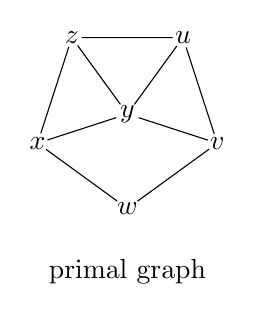
\begin{tikzpicture}[scale=.8]
 \tikzstyle{every circle node}=[circle, inner sep=0pt]
            \draw (0,0)    node[circle] (y) {$y$} 
                  +(90-36:1.5cm)  node[circle] (u) {$u$} 
                  +(90-72-36:1.5cm)  node[circle] (v) {$v$} 
                  +(90-2*72-36:1.5cm)  node[circle] (w) {$w$} 
                  +(90-3*72-36:1.5cm)  node[circle] (x) {$x$} 
                  +(90-4*72-36:1.5cm)  node[circle] (z) {$z$}; 
             \draw (u) -- (z) -- (x) -- (w) -- (v) -- (u);
             \draw (y) -- (u) (y) -- (z) (y) -- (x) (y)--(v);     
             \draw (0,-2.5) node (text) {primal graph};
  \end{tikzpicture}\hfill% 
 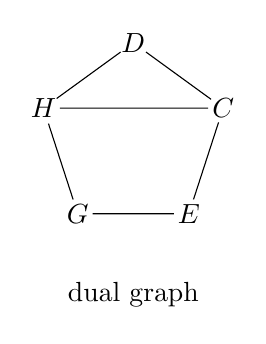
\begin{tikzpicture}[scale=.8]
 \tikzstyle{every circle node}=[circle, inner sep=0pt]
            \draw (0,0)    node[circle] (y) {} 
                  +(90:1.5cm)  node[circle] (c2) {$D$} 
                  +(90+72:1.5cm)  node[circle] (c5) {$H$} 
                  +(90+2*72:1.5cm)  node[circle] (c4) {$G$} 
                  +(90+3*72:1.5cm)  node[circle] (c3)  {$E$} 
                  +(90+4*72:1.5cm)  node[circle] (c1) {$C$}; 
             \draw (c5) -- (c1) -- (c2) -- (c5) -- (c4) -- (c3) -- (c1);
             \draw (0,-2.5) node (text) {dual graph};
  \end{tikzpicture}\hfill%
        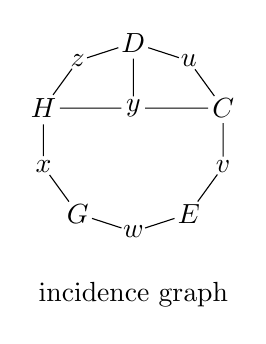
\begin{tikzpicture}[scale=.8]
 \tikzstyle{every circle node}=[circle, inner sep=0pt]
            \draw (0,0)    node[circle] (center) {} 
                  +(90+0*36:1.5cm)  node[circle] (2) {$D$} 
                  +(90+1*36:1.5cm)  node[circle] (z) {$z$} 
                  +(90+2*36:1.5cm)  node[circle] (5) {$H$} 
                  +(90+3*36:1.5cm)  node[circle] (x)  {$x$} 
                  +(90+4*36:1.5cm)  node[circle] (4)  {$G$} 
                  +(90+5*36:1.5cm)  node[circle] (w)  {$w$} 
                  +(90+6*36:1.5cm)  node[circle] (3)  {$E$} 
                  +(90+7*36:1.5cm)  node[circle] (v)  {$v$} 
                  +(90+8*36:1.5cm)  node[circle] (1)  {$C$} 
                  +(90+9*36:1.5cm)  node[circle] (u)  {$u$}; 

     \draw (intersection of 1--5 and w--2) node[circle](y){$y$};  

      \draw (u) -- (1) (u) -- (2);
      \draw (v) -- (1) (v) -- (3);
      \draw (w) -- (3) (w) -- (4);
      \draw (x) -- (4) (x) -- (5);
      \draw (y) -- (1) (y) -- (5) (y)--(2);
      \draw (z) -- (2) (z) -- (5);
      \draw (0,-2.5) node (text) {incidence graph};
    \end{tikzpicture}\hspace*{5mm}%

\noindent
This gives rise to parameters \alert{primal treewidth}, \alert{dual treewidth,} and
\alert{incidence treewidth.}

\end{frame}

\begin{frame}
	\slides{\frametitle{Formally}}
	
	\begin{definition}
		Let $F$ be a CNF formula with variables $\var(F)$ and clauses $\cla(F)$.\\
		The \alert{primal graph} of $F$ is the graph with vertex set $\var(F)$ where two variables are adjacent if they appear together in a clause of $F$.\\
		The \alert{dual graph} of $F$ is the graph with vertex set $\cla(F)$ where two clauses are adjacent if they have a variable in common.\\
		The \alert{incidence graph} of $F$ is the bipartite graph with vertex set $\var(F) \cup \cla(F)$ where a variable and a clause are adjacent if the variable appears in the clause.\\
		The \alert{primal treewidth}, \alert{dual treewidth}, and \alert{incidence treewidth} of $F$ is the treewidth of the primal graph, the dual graph, and the incidence graph of $F$, respectively.
	\end{definition}
\end{frame}
 
\begin{frame}
  \frametitle{Incidence treewidth is most general}
  \begin{lemma}
   The incidence treewidth of $F$ is at most the primal treewidth of $F$ plus $1$.
  \end{lemma}
  \begin{proof}
    Start from a tree decomposition $(T,\gamma)$ of the primal graph with minimum width.\\
	For each clause $C$:
	\begin{itemize}
		 \item There is a node $t$ of $T$ with
		 $\var(C)\subseteq \gamma(t)$, since $\var(C)$ is a clique in the primal graph.
		 \item Add to $t$ a new neighbor $t'$ with $\gamma(t')=\gamma(t)\cup
		 \{C\}$.
    \end{itemize}
  \end{proof}
\end{frame}

\begin{frame}
	\slides{\frametitle{Incidence treewidth is most general II}}
  \begin{lemma}
    The incidence treewidth of $F$ is at most the dual treewidth of $F$ plus $1$.
  \end{lemma}
  \pause
  \noindent
  Primal and dual treewidth are incomparable. 
    \begin{itemize}
    \item One big clause alone gives
    large primal treewidth.
  \item  $\{\{x,y_1\},\{x,y_2\},\dots,\{x,y_n\}\}$
    gives large dual treewidth.
    \end{itemize}
\end{frame}


\begin{frame}
	\frametitle{\textsc{SAT} parameterized by treewidth}
	\pbDefNoPara{\textsc{Sat}}{A CNF formula $F$}{Is there an assignment of truth values to $\var(F)$ such that $F$ evaluates to \textsf{true}?}
	
	\noindent
	\textbf{Note}: If \textsc{Sat} is \FPT\ parameterized by incidence treewidth, then \textsc{Sat} is \FPT\ parameterized by primal treewidth and by dual treewidth.
\end{frame}


\begin{frame}
  \frametitle{{SAT is FPT for parameter incidence treewidth}}

\noindent
 CNF Formula $F=C\wedge D\wedge E\wedge G\wedge H$ where  
	$C= (u \vee v \vee \neg y)$, 
	$D= (\neg u\vee z \vee y)$, 
	$E= (\neg v\vee w)$, 
	$G= (\neg w\vee x)$, 
	$H= (x\vee y\vee \neg z)$ 

{Auxiliary graph:}
{
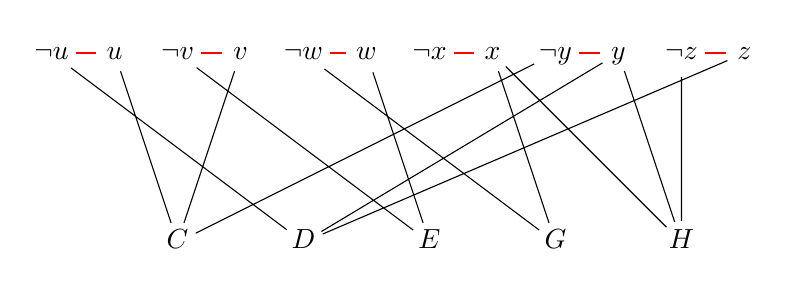
\begin{tikzpicture}[scale=.8]
 \tikzstyle{every node}=[circle, inner sep=0pt]
 \pgfsetbaseline{-1.5cm}

\draw (0,0) node (nu) {\strut $\neg u$};
\draw (1,0) node (u) {\strut $u$};
\draw (2,0) node (nv) {\strut $\neg v$};
\draw (3,0) node (v) {\strut $v$};
\draw (4,0) node (nw) {\strut $\neg w$};
\draw (5,0) node (w) {\strut $w$};
\draw (6,0) node (nx) {\strut $\neg x$};
\draw (7,0) node (x) {\strut $x$};
\draw (8,0) node (ny) {\strut $\neg y$};
\draw (9,0) node (y) {\strut $y$};
\draw (10,0) node (nz) {\strut $\neg z$};
\draw (11,0) node (z) {\strut $z$};

\draw (2,-3) node (C) {\strut $C$};
\draw (4,-3) node (D) {\strut $D$};
\draw (6,-3) node (E) {\strut $E$};
\draw (8,-3) node (F) {\strut $G$};
\draw (10,-3) node (G) {\strut $H$};


\draw[thick, red] 
(nu)--(u) 
(nv)--(v) 
(nw)--(w) 
(nx)--(x) 
(ny)--(y) 
(nz)--(z);

\draw


(u)--(C)--(v) (ny)--(C)
(nu)--(D)--(z)
(nv)--(E)--(w)
(nw)--(F)--(x)
(x)--(G)--(y)--(D) (nz)--(G);

  \end{tikzpicture}
}
  \begin{itemize}
  \item 
MSO Formula: \textsl{``There exists an independent set of literal vertices that
dominates all the clause vertices.''}

\item The treewidth of the auxilary graph is at most twice the treewidth of the
incidence graph plus one.
  \end{itemize}

\end{frame}


\begin{frame}
  \frametitle{FPT via MSO}
   \begin{theorem}
   	\textsc{Sat} is \FPT\ for each of the following parameters: primal treewidth, dual treewidth, and incidence treewidth.
   \end{theorem} 
\end{frame}

\section{Dynamic Programming over Tree Decompositions}

\begin{frame}
	\frametitle{Coucelle's theorem: discussion}
	
	\noindent
	Advantages of Courcelle's theorem:
	\begin{itemize}
		\item general, applies to many problems
		\item easy to obtain \FPT\ results
	\end{itemize}
	Drawback of Courcelle's theorem
	\begin{itemize}
		\item the resulting running time depends non-elementarily on the treewidth $t$ and the length $\ell$ of the MSO-sentence, i.e., a tower of $2$'s whose height is $\omega(1)$
		\begin{align*}
		 2^{2^{2^{{\iddots}^{t+\ell}}}}
		\end{align*}
	\end{itemize}
\end{frame}

\begin{frame}{Dynamic progamming over tree decompositions}
	
	\noindent
	Idea: extend the algorithmic methods that work for trees to tree decompositions.
	
	\noindent
	\begin{description}
		\item[Step 1] Compute a minimum width tree decomposition using Bodlaender's algorithm
		\item[Step 2] Transform it into a standard form making computations easier
		\item[Step 3] Bottom-up Dynamic Programming (from the leaves of the tree decomposition to the root)
	\end{description}
\end{frame}

\begin{frame}
  \frametitle{Nice tree decomposition}

  \noindent
  A \emph{nice} tree decomposition $(T,\gamma)$ is rooted and has only 4 kinds of nodes:
  \begin{itemize}
   \item \emph{leaf node}: leaf $t$ in $T$ and $|\gamma(t)|=1$
   \item \emph{introduce node}: node $t$ with one child $t'$ in $T$ and $\gamma(t) = \gamma(t') \cup \{x\}$
   \item \emph{forget node}: node $t$ with one child $t'$ in $T$ and $\gamma(t) = \gamma(t') \setminus \{x\}$
   \item \emph{join node}: node $t$ with two children $t_1,t_2$ in $T$ and $\gamma(t) = \gamma(t_1) = \gamma(t_2)$
  \end{itemize}
  Every tree decomposition of width $w$ of a graph $G$ on $n$ vertices can be transformed into a nice tree decomposition of width $w$ and $O(w\cdot n)$ nodes in polynomial time \cite{Kloks94}.

\end{frame}

\subsection{SAT}

\begin{frame}
  \frametitle{Dynamic programming: primal treewidth}

  \begin{itemize}
   \item Compute a nice tree decomposition $(T,\gamma)$ of $F$'s primal graph with minimum width rooted at some node $r$ \cite{Bodlaender96, Kloks94}
   \pause
   \item Notation
   \begin{itemize}
   \item $T_t$ is the subtree of $T$ rooted at node $t$
   \item $\gamma_\downarrow (t) = \{ x\in \gamma(t') : t' \in V(T_t)\}$ is the set of vertices/variables in $T_t$'s bags
   \item $F_\downarrow (t) = \{ C\in \cla(F) : \var(C) \subseteq \gamma_\downarrow (t) \}$ is the set of clauses containing only variables from $\gamma_\downarrow$
   \item For a clause $C\in \cla(F)$ and an assignment $\tau : S\rightarrow \{0,1\}$ to a subset of variables $S\subseteq \var(F)$, we can efficiently compute
   \begin{align*}
   \falsifies(\tau,C) &= \begin{cases}
   1 & \text{if $\tau$ sets each literal of $C$ to 0}\\
   0 & \text{otherwise.}
   \end{cases}
   \end{align*}
   \end{itemize}
   \pause
   \item For each node $t$ and each assignment $\tau: \gamma(t) \rightarrow \{0,1\}$, our DP algorithm will compute
         \begin{align*}
         \sat(t,\tau) = \begin{cases}1 & \text{if $\tau$ can be extended to a}\\ & \text{satisfying assignment of $F_\downarrow (t)$}\\0 & \text{otherwise.} \end{cases}
         \end{align*}
  \end{itemize}

\end{frame}


\begin{frame}
  \slides{\frametitle{DP: primal treewidth II}}

  \slides{%
  \begin{align*}
     \sat(t,\tau) = \begin{cases}1 & \text{if $\tau$ can be extended to a}\\ & \text{satisfying assignment of $F_\downarrow (t)$}\\0 & \text{otherwise.} \end{cases}
  \end{align*}
  }
  \noindent

  \begin{itemize}
   \item \emph{leaf node}: $|\gamma(t)|=1$\pause
   \begin{align*}
   \sat(t,\tau) &= \begin{cases} 0 & \text{if $\exists C\in \cla(F)$ s.t. $\falsifies(\tau,C)$}\\1 & \text{otherwise}\end{cases}
   \end{align*}
   \pause
   \item \emph{introduce node}: $\gamma(t) = \gamma(t') \cup \{x\}$.
   \pause
          \begin{align*}
           %\slides{\color{Blue}}
           \sat(t,\tau) = \sat(t', \tau|_{\gamma(t')}) 
           \; \wedge \;  (\nexists C\in F : \falsifies(\tau,C)).
          \end{align*}
  \end{itemize}

\end{frame}

\begin{frame}
  \slides{\frametitle{DP: primal treewidth III}}

  \begin{itemize}
  	\item \emph{forget node}: $\gamma(t) = \gamma(t') \setminus \{x\}$.\pause
  	\begin{align*}
  	\sat(t, \tau) &= \sat(t', \tau_{x=0})\vee \sat(t', \tau_{x=1}),\\
  	\text{where } \tau_{x=a}(y) &= \begin{cases} a & \text{if $y=x$}\\ \tau(y) & \text{otherwise}\end{cases}
  	\end{align*}
  	\pause
  	\item \emph{join node}: $\gamma(t) = \gamma(t_1) = \gamma(t_2)$\pause
  	  	\begin{align*}
  	  	\sat(t, \tau) &= \sat(t_1, \tau) \wedge \sat(t_2, \tau).
  	  	\end{align*}
  \end{itemize}
  
  \pause
  \begin{itemize}
   \item Finally: $F$ is satisfiable iff $\exists \tau: \gamma(r) \rightarrow \{0,1\}$ such that $\sat(r,\tau)=1$
   \item Running time: $O^*(2^k)$, where $k$ is the primal treewidth of $F$
   \item Also extends to computing the number of satisfying assignments
  \end{itemize}

\end{frame}


\begin{frame}
  \frametitle{Direct Algorithms}
  
  \noindent
  Known treewidth based algorithms for \textsc{Sat}:
  \begin{center}
  \begin{tabular}{c@{\qquad} c@{\qquad} c}
    $k= {}$primal tw & $k= {}$dual tw & $k= {}$incidence tw\\[4pt]
    $O^*(2^{k})$&
    $O^*(2^{k})$&
    $O^*(2^{k})$\\
  \end{tabular}
\end{center}
  \begin{itemize}
  \item These algorithms all count the number of satisfying assignments
  \item The algorithm for incidence treewidth \cite{SlivovskyS20} uses Fast Subset Convolution
  \end{itemize}
\end{frame}


\subsection{CSP}

\begin{frame}{Constraint Satisfaction Problem}
	
	\pbDefNoPara{CSP}{A set of variables $X$, a domain $D$, and a set of constraints $C$}{Is there an assignment $\tau:X\rightarrow D$ satisfying all the constraints in $C$?}
	
	\noindent
	A \alert{constraint} has a \alert{scope} $S=(s_1,\dots,s_r)$ with $s_i\in X, i\in \{1,\dots,r\}$, and a \alert{constraint relation} $R$ consisting of $r$-tuples of values in $D$.\\ An assignment $\tau: X\rightarrow D$ \alert{satisfies} a constraint $c=(S,R)$ if there exists a tuple $(d_1,\dots,d_r)$ in $R$ such that $\tau(s_i)=d_i$ for each $i\in \{1,\dots,r\}$.
\end{frame}

\begin{frame}
  \frametitle{Bounded Treewidth for Constraint Satisfaction}
  \begin{itemize}
  \item Primal, dual, and incidence graphs are defined similarly as for \textsc{Sat}.
  \end{itemize}
  \begin{theorem}[\cite{GottlobSS02}]
  	CSP is \FPT\ for parameter primal treewidth if $|D|=O(1)$.
  \end{theorem}
  \begin{itemize}
  \item What if domains are unbounded?
  \end{itemize}
\end{frame}

\begin{frame}
  \frametitle{Unbounded domains}
  \begin{theorem}
  	CSP is
      $\W[1]$-hard for parameter primal treewidth.
  \end{theorem}
  \pause
  \begin{proof}[Proof Sketch]
  	Parameterized reduction from \textsc{Clique}.\\
    Let $(G=(V,E),k)$  be an instance of \textsc{Clique}.\\
    Take $k$ variables $x_1,\dots,x_k$, each with domain $V$.\\
    Add $\binom{k}{2}$ binary constraints $E_{i,j}$, $1\leq i < j \leq k$.\\
    A constraint $E_{i,j}$ has scope $(x_i,x_j)$ and its constraint relation contains the tuple $(u,v)$ if $uv\in E$.\\
    The primal treewidth of this CSP instance is $k-1$.
  \end{proof}
\end{frame}


\section{Further Reading}

\begin{frame}
 \slides{\frametitle{Further Reading}}

  \begin{itemize}
   \item Chapter 7, \emph{Treewidth} in \cite{CyganFKL+15}
%   Marek Cygan, Fedor V.\ Fomin, \L ukasz Kowalik, Daniel Lokshtanov, D{\'a}niel Marx, Marcin Pilipczuk, Micha\l Pilipczuk, and Saket Saurabh. Parameterized Algorithms. Springer, 2015.
   \item Chapter 5, \emph{Treewidth} in \cite{FominK10}
%         Fedor V. Fomin and Dieter Kratsch. Exact Exponential Algorithms. Springer, 2010.
   \item Chapter 10, \emph{Tree Decompositions of Graphs} in \cite{Niedermeier06}
%         Rolf Niedermeier. Invitation to Fixed Parameter Algorithms. Oxford University Press, 2006.
   \item Chapter 10, \emph{Treewidth and Dynamic Programming} in \cite{DowneyF13}
%         Rodney G. Downey and Michael R. Fellows. Fundamentals of Parameterized Complexity. Springer, 2013.
   \item Chapter 13, \emph{Courcelle's Theorem} in \cite{DowneyF13}
%         Rodney G. Downey and Michael R. Fellows. Fundamentals of Parameterized Complexity. Springer, 2013.
  \end{itemize}

\end{frame}


\begin{frame}[t, allowframebreaks]
	\slides{\frametitle{References}}
	\printbibliography
\end{frame}

\end{document}
